% --------------------------------------------------------------------------------

\begin{exercise}[\textbf{Random walk of a robot}]

A robot is placed at the origin (the point $(0, 0)$) on a two-dimension integer grid (see the figure below).
Denote the position of the robot by $(x, y)$.
The robot can either move right to $(x + 1, y)$ or move up to $(x, y + 1)$.

\begin{center}
    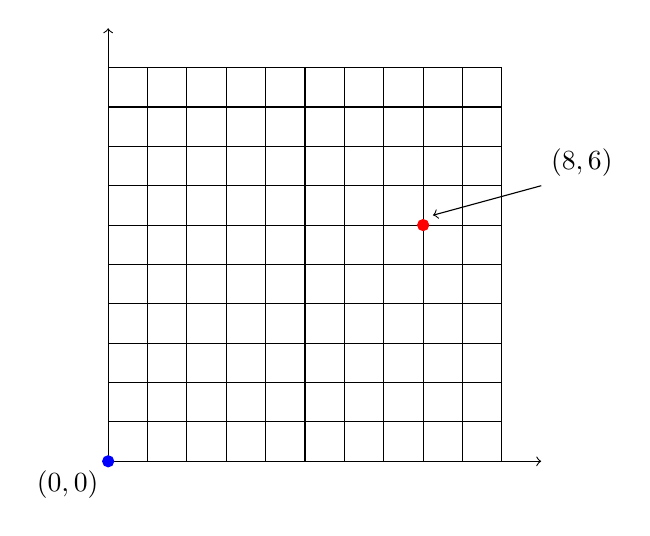
\begin{tikzpicture}[scale = 0.5]

        \draw [->] (0, 0) -- (0, 11);
        \draw [->] (0, 0) -- (11, 0);
        \draw (0, 0) grid (10, 10);

        \filldraw [color = blue] (0, 0) circle (4pt);
        \draw node [below left] {$(0, 0)$};

        \filldraw [color = red] (8, 6) circle (4pt);
        \draw [->] (11, 7) node [above right] {$(8, 6)$} -- (8.25, 6.25);

    \end{tikzpicture}
\end{center}

\begin{enumerate}[label = (\alph*)]

    \item Suppose each time the robot randomly moves right or up with equal chance.
    What is the probability that the robot will ever reach the point $(8, 6)$?

    \item Suppose another robot has a $\frac{2}{3}$ chance to move right and a $\frac{1}{3}$ chance to move up when $x + y$ is even, otherwise it has a $\frac{1}{4}$ chance to move right and a $\frac{3}{4}$ chance to move up.
    It stops whenever $|x - y| \geq 2$.
    Find the probability that $x - y = 2$ when it stops.

\end{enumerate}

\end{exercise}

% --------------------------------------------------------------------------------

\begin{solution}

\phantom{}

\begin{enumerate}[label = (\alph*)]
  \item The robot increases the sum $x + y$ by one in every step. That means, it can only
  reach the point $(8,6)$ in the fourteenth step and there are fourteen different places,
  where it can end up after fourteen steps.
  Therefore the probability can be calculated by a binomial distribution
  with $p = \frac{1}{2}$ and $n = 14$.
  \begin{align*}
    \P(\text{robot lands on} (8,6)) = \frac{1}{2^{14}}\binom{8}{14} = \frac{3003}{16384} \approx 0.1833.
  \end{align*}
  \item The robot can leave the corridor $|x - y| < 2$ only on every even turn.
  Every even turn, there are three possibilities:
  \begin{itemize}
    \item He stays on the main diagonal: $x = y$.
    \item He leaves the corridor at the upper end: $y - x = 2$.
    \item He leaves the corridor at the lower end: $x - y = 2$.
  \end{itemize}

  Now let's suppose the robot is already at the point $(z,z)$.
  What are the probabilities of arriving at $(z+1,z+1), (z+2,z)$ and $(z,z+2)$
  in the next two turns respectively?

  For the first turn $x+y = 2z$ is even, for the second turn $x+y=2z+1$ is even
  independent of the choice for the first move. Therefore

  \begin{align*}
    \P((z+2,z)|(z,z)) &= \frac{2}{3}\frac{1}{4} = \frac{2}{12} \\
    \P((z,z + 2)|(z,z)) &= \frac{1}{3}\frac{3}{4} = \frac{3}{12} \\
    \P((z+1,z+1)|(z,z)) &= 1 - \frac{2}{12} - \frac{3}{12} = \frac{7}{12}.
  \end{align*}

  Now we can calculate the probability of the robot leaving the corridor at the lower
  end by

  \begin{align*}
    \P(x-y=2 \text{ at the end}) &= \sum_{k=0}^\infty \frac{2}{12}\left(\frac{7}{12}\right)^k \\
    &= \frac{2}{12}\frac{1}{1 - \frac{7}{12}} = \frac{2}{5}.
  \end{align*}

\end{enumerate}



\end{solution}

% --------------------------------------------------------------------------------
